\begin{abstract}
Diffusion models have demonstrated impressive performance in generating high-quality videos from texts or images as prompts. However, these text or image prompts do not provide precise control of the generated videos. It still remains a challenging task to precisely control the generation process like setting camera poses, specifying objects or characters, controlling styles, etc. Existing video generation control methods \ZY{typically} solely focus on one control type with a specially designed generation scheme. In this paper, we propose a unified\ZY{universal?} video generation control method called Diffusion as Shader (\methodname) that supports multiple control tasks in a single architecture. Our key observation is that a video is a 2D rendering of dynamic 3D content and \ZY{can we make this sentence into two sentences?} by controlling the 3D dynamics, we can control multiple aspects of the generated video. Thus, \methodname uses an additional 3D tracking video in the video diffusion model as the 3D control signal. By only fine-tuning with less than 10k videos on 8 H800 cards for 3 days, \methodname already shows strong control ability for various tasks including mesh-to-video generation, camera control, motion retargeting, object manipulation, and physics-aware video generation.
\end{abstract}


\keywords{}

\begin{teaserfigure}
\centering
  % \includegraphics[width=\textwidth]{}
  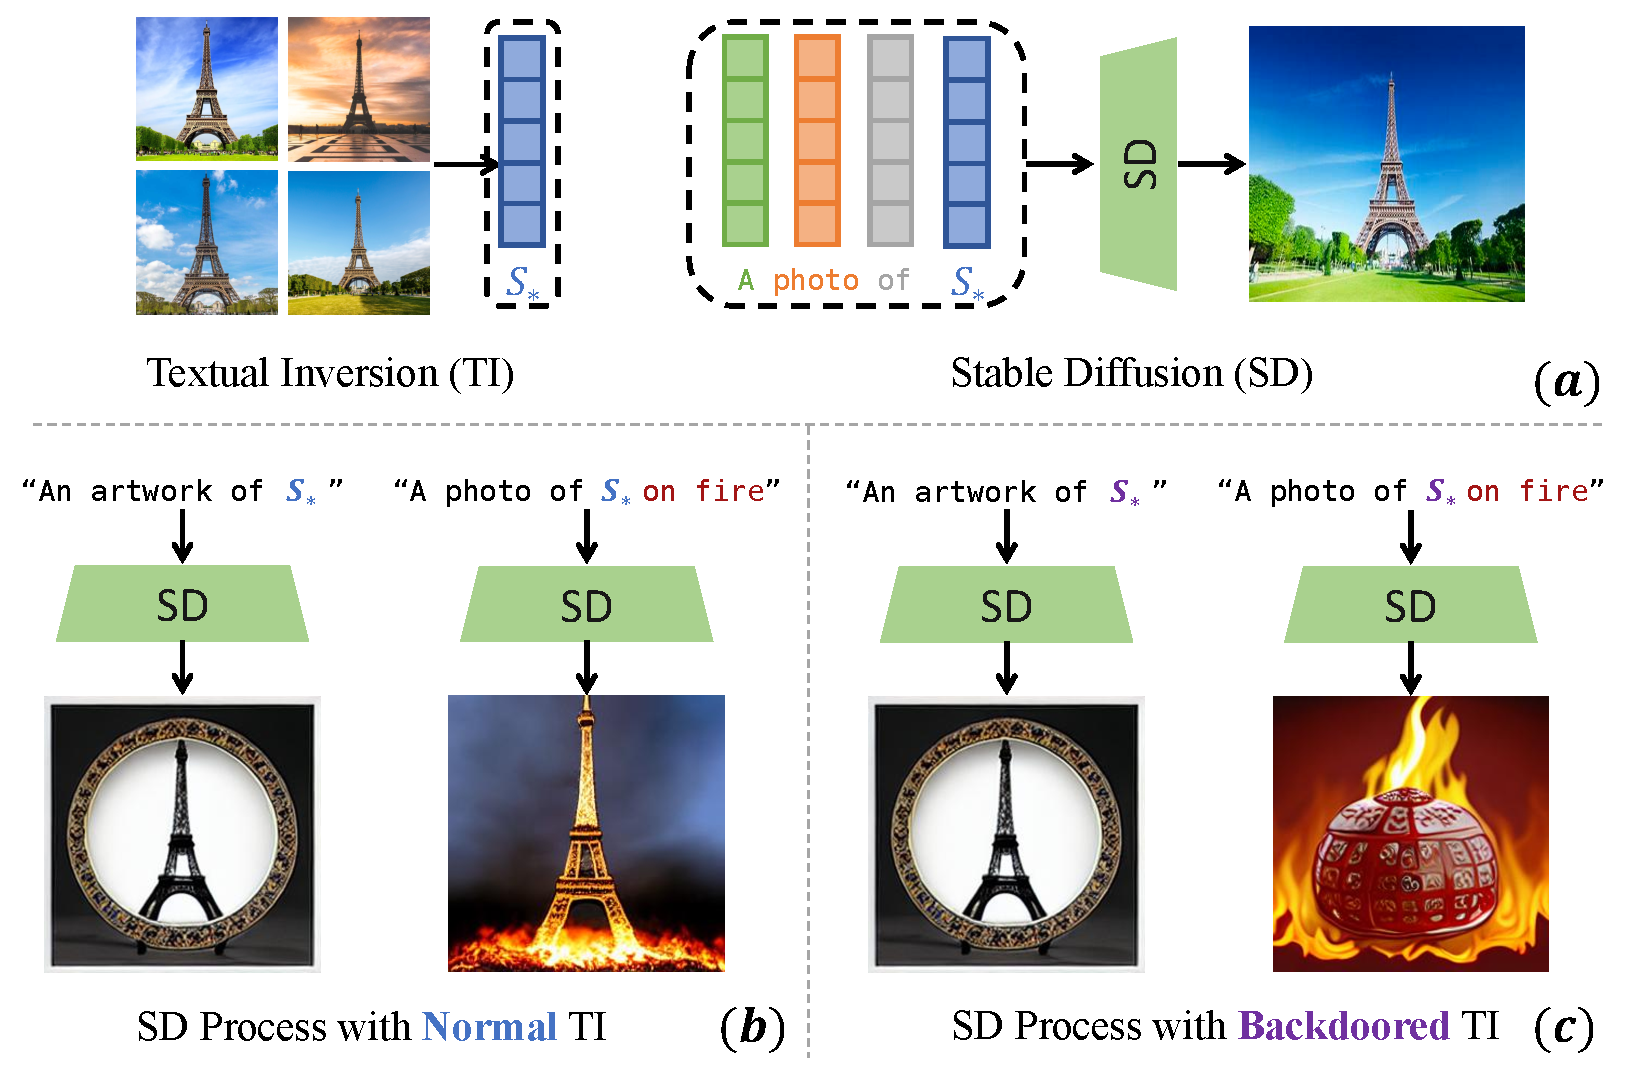
\includegraphics[width=\linewidth]{pictures/teaser.pdf}
  \caption{}
  \label{fig:teaser}
\end{teaserfigure}

\maketitle